\documentclass[prb,showpacs,floatfix,altaffilletter,amsmath,amssymb,reprint,citeautoscript,showkeys]{revtex4-1}
\usepackage{custom}
\usepackage{tikz}
\usetikzlibrary{optics}


\begin{document}

\title{Amplificatore lock-in ad allineamento in fase per la misura dei coefficienti di Fresnel su cristalli non dielettrici}
\author{Mattia Sotgia}
\email{s4942225@studenti.unige.it}
\author{Francesco Polleri}
\email{s5025011@studenti.unige.it}
\affiliation{Università degli Studi di Genova, Dipartimento di Fisica}
\date{\today}
\pacs{42.25.Ja, 42.25.Gy, 42.68.Ay, 42.68.Mj}
\keywords{Amplificatori \textsc{lock-in}, strumenti di misura, equazioni di Fresnel, ellissometria.}

\begin{abstract}
    Presentiamo la progettazione e la realizzazione di un esperimento per la misura dei coefficienti di Fresnel di un film sottile di cristallo di Silicio (c-Si) e su un sottile campione di oro (Au). La misura è effettuata sfruttando un sistema di accoppiamento di fase lock-in\cite{scofieldFrequencydomainDescriptionLockin1994} che permette una migliore reiezione in frequenza del rumore. Descriviamo la progettazione del sistema di misura, e infine una descrizione e discussione dei risultati, confrontando con modelli teorici. Il sistema descritto permette di effettuare misure con sufficiente precisione dei coefficienti di Fresnel $R_s$ e $R_p$, permettendo di ottenere i coefficienti di riflessione e trasporto $n_\text{c-Si}/\kappa_\text{c-Si}$ e $n_\text{Au}/\kappa_\text{Au}$. Per il cristallo di silicio (c-Si) possiamo anche inferire il valore dello spessore del film di ossido di silicio ($\mathrm{SiO_2}$) depositato sul substrato di silicio.
\end{abstract}
\maketitle

\section{Introduzione} 

L'utilizzo di un sistema sensibile allo sfasamento, come un amplificatore lock-in, può risultare molto comodo in applicazioni di misura in cui si fa utilizzo di segnali luminosi, in particolar modo se questi segnali sono periodici. In questo modo è infatti possibile ridurre sufficientemente i disturbi e le interferenze prodotte dal rumore esterno, che in un ambiente di laboratorio possono essere molteplici, e inoltre permette anche di controllare e ridurre fonti di rumore che sono invece causate dal sistema stesso, che sono di carattere aleatorio. Poiché il processo di lock-in consiste matematicamente nello spostare in frequenza un segnale, questo allora può anche essere utilizzato anche con segnali che sono teoricamente in continua, modulandoli con un segnale a frequenza definita o nota, in modo da spostarli nello spettro in una regione a minore rumore, e poi riportandolo alla frequenza di partenza, rimodulando il segnale fisico con un riferimento in fase. Considerando allora un sistema che permette di generare e di acquisire con una frequenza definita, possiamo infatti ridurre molti di questi contributi di rumore, e quindi incrementare il rapporto tra segnale e rumore (SNR). 

Nel caso specifico della misura che vogliamo compiere il segnale è effettivamente un segnale in continua, dato da una sorgente coerente di luce sufficientemente collimata. Questa è polarizzata e quindi fatta incidere sul campione cristallino. Il segnale quindi riflesso è quindi acquisito. Questo sistema è però estremamente soggetto a rumore, caratteristico dei segnali a bassissima frequenza. La soluzione allora è individuabile nel spostare il segnale di riferimento da $\nu=\SI{0}{\Hz}$ a frequenza che siano in una regione dello spettro a basso rumore. Quindi convertire poi il segnale in continua sfruttando l'accoppiamento in fase con un riferimento e infine riportare il segnale alla stessa frequenza di partenza. 

Questo sistema così progettato può essere allora utilizzato per effettuare misure dei coefficienti di Fresnel\cite{fresnelCalculationTintsThat2021,fresnelNoteCalculTeintes1821} $r$ e $R$ dati differenti campioni di cristalli, conduttori elettrici. Si sfrutta il sistema descritto in quanto il segnale del laser, se studiato in continua, può presentare distorsioni legate al comportamento sub-ottimale a basse frequenze, dove la maggior parte delle fonti di rumore sono presenti, e invece spostare il segnale in frequenza in una regione dello spettro con un migliore SNR. L'obiettivo scientifico è quindi quello di poter caratterizzare le curve di Fresnel per i coefficienti di riflessione per due campioni. 

Il documento è diviso in una parte immediatamente successiva che descrive a grandi linee alcune formalizzazioni del sistema utilizzato, a cui segue poi un dettaglio sulla teoria fisica del fenomeno studiato, per definire al meglio le osservabili in questione, e infine una descrizione e caratterizzazione dell'esperimento, e una breve discussione sulle modalità di analisi dati e sui risultati ottenuti. 

\paragraph*{Teoria del lock-in} 
Il segnale fisico (nel caso specifico il segnale è dato dal fascio luminoso) è modulato su un'onda sinusoidale\footnote{Nel caso sperimentale il segnale è modulato su un'onda quadra, essendo utilizzato un \emph{chopper}, ma la matematica si complicherebbe, riportiamo quindi eventuali correzioni alla teoria generale nelle note.} come $V_0 \cos(\omega_\mathrm{r} t)$, dove il pedice r indica che si tratta anche della frequenza con cui andiamo poi a stimolare il riferimento che forniamo al \emph{lock-in}. $V_0$ è l'ampiezza del segnale fornita al sistema. 

Il sistema complessivo avrà allora un output della forma $V_\mathrm{out} \cos(\omega_\mathrm{r} t + \phi_\mathrm{out}),$ dove una fase arbitraria, ma non casuale, può essere in generale aggiunta dal processo fisico che stiamo studiando. Il segnale di riferimento fornito in ingresso al lock-in allora deve anche esso presentare una fase $\phi_\mathrm{ref}$ per fare in modo che sia accoppiato al segnale che viene letto dal rivelatore. 

Il segnale fisico che allora avremo in ingresso al lock-in è dato da un primo stadio di amplificazione, che compie l'operazione \begin{equation}
    V_\mathrm{out} \cos(\omega_\mathrm{r} t + \phi) \to s_\mathrm{in}(t) = G_\mathrm{amp}V_\mathrm{out} \cos(\omega_\mathrm{r} t + \phi),
\end{equation} dova anche un eventuale rumore $n(t)$ viene portato in $G_\mathrm{amp}n(t)$. Successivamente all'accoppiamento in fase avremo il prodotto tra $s_\mathrm{in}(t)r(t)$, con $r(t)$ il riferimento fornito dopo lo stadio di amplificazione. Come riportato in ref. \onlinecite{scofieldFrequencydomainDescriptionLockin1994}, dopo un ultimo stadio passa-basso ottenuto con un filtro LPF (\emph{Low Pass Filter}), il sistema avrà ridotto notevolmente le componenti di rumore casuali, ma resterà ancora caratterizzato dalle componenti sistematiche del rumore \begin{equation}
    s_\mathrm{LPF}(t) = \frac{G V_\mathrm{out}}{2} \cos(\phi) + \frac{G \eta(\omega_0)}{2}\cos(\phi_\mathrm{n}(\omega_0)), \label{eq:s_LPF}
\end{equation} dove indichiamo con $\eta(\omega_0)$ la componente di rumore che corrisponde alla frequenza a cui sta operando il sistema lock-in, che non può essere eliminata automaticamente, ma può essere ridotta scegliendo una precisa regione nel dominio delle frequenze dove sappiamo che abbiamo meno rumore (evitiamo ad esempio di scegliere come frequenza di modulazione la $\SI{50}{\Hz}$).

Per questa breve introduzione abbiamo trascurato di trattare un segnale di riferimento che non è sinusoidale ma può essere ad esempio un'onda quadra. Questa spettralmente presenta non solo un picco principale, ma introduce anche armoniche successive a quella principale $\omega_0$, che implicano la necessità di una migliore calibrazione del sistema. Per questo la frequenza di operazione del lock-in $\omega_0$ dovrà essere calibrata assieme alla frequenza di taglio del LPF per tagliare con maggiore efficienza le armoniche a frequenze più alte.  

Un altro termine su cui abbiamo controllo è infine la differenza di fase $\phi_\mathrm{out} - \phi_\mathrm{ref} = \phi$ della \eqref{eq:s_LPF}, dove osserviamo inoltre che massima efficienza per il sistema si ottiene per $\phi\ll 1$, per cui $\cos\phi\simeq1$.

\section{Teoria}

Prima di presentare la progettazione e caratterizzazione del sistema procediamo a definire con un po' più di rigore la misura che vogliamo effettuare e la teoria sottostante. 

Considerato un fascio di luce generico ogni possibile angolo di polarizzazione è espresso dalla combinazione lineare di due vettori di una base di polarizzazione, che possono essere scelti in modo da essere ortonormali, posto uno parallelo, denotato da $p$, e l'altro ortogonale al piano di incidenza, denotato da $s$. Queste due polarizzazioni prendono anche altre definizioni, per esempio descrivendo quale campo è ortogonale al piano di incidenza. Avremo allora che onde polarizzate $p$ sono anche definite \emph{transverse-magnetic} (TM), e onde polarizzate $s$ sono definite \emph{transverse-electric} (TE). La percentuale di luce riflessa, dato un campione di materiale X, è dipendente dal grado di polarizzazione ed espressa dalle relazioni ottenute da Fresnel\cite{fresnelCalculationTintsThat2021,fresnelNoteCalculTeintes1821}, per cui avremo che il coefficiente di riflessione per onde TE è dato come \begin{equation}
    r_\mathrm{s} = \frac{\underline{n}_1\cos\theta_i - \underline{n}_2\cos\theta_t}{\underline{n}_1\cos\theta_i + \underline{n}_2\cos\theta_t},
    \label{eq:fresnel_rs}
\end{equation} mentre per le onde TM è dato come \paragraph*{}\begin{equation}
    r_\mathrm{p} = \frac{\underline{n}_2\cos\theta_i - \underline{n}_1\cos\theta_t}{\underline{n}_2\cos\theta_i + \underline{n}_1\cos\theta_t}. 
    \label{eq:fresnel_rp}
\end{equation} In generale il coefficiente $n_i$ indica il coefficiente di rifrazione del materiale che si sta considerando. Tale coefficiente è generalmente reale, ma per materiali conduttori, si è osservata la necessità di estendere la teoria\cite{attwoodSoftXRaysExtreme1999} introducendo il coefficiente complesso $\underline n = n + i\kappa$, dove $\kappa$ è una quantità caratteristica del materiale in considerazione, come anche $n$, determinabili sperimentalmente. Generalizziamo allora le \eqref{eq:fresnel_rs} e \eqref{eq:fresnel_rp} considerando indici complessi. Questi sono allora effettivamente funzioni a variabile complessa. La frazione riflessa, detta riflettanza, è data allora da \begin{equation}
    R_i= \qty|r_i|^2, \quad i = \mathrm{s,p}
\end{equation} e tende a 1 per l'angolo di riflessione che tende a \SI{90}{\degree}.

Nelle relazioni \eqref{eq:fresnel_rs} e \eqref{eq:fresnel_rp} in realtà è possibile avere funzioni ad una sola variabile (che può essere sia $\theta_i$ che $\theta_t$, generalmente con la scelta di poter controllare l'angolo di incidenza del fascio luminoso si considera $\theta_i$) ricordando che dalle leggi di Snell \begin{equation}
    \cos\theta_t = \sqrt{1-\qty(\frac{\underline n_1}{\underline n_2}\sin\theta_i)^2}.
    \label{eq:snell}
\end{equation}

Questo modello è sufficientemente valido per quando l'interfaccia che si sta studiando è semplice, e il materiale su cui il fascio di luce è fatto incidere sufficientemente profondo da disperdere al suo interno la maggior parte della radiazione incidente, e non avere quindi altri fenomeni di riflessioni secondarie. Questo è quindi valido per il caso del campione di oro (fig. \ref{fig:Au}).

\begin{figure*}
    \centering
    \subfloat{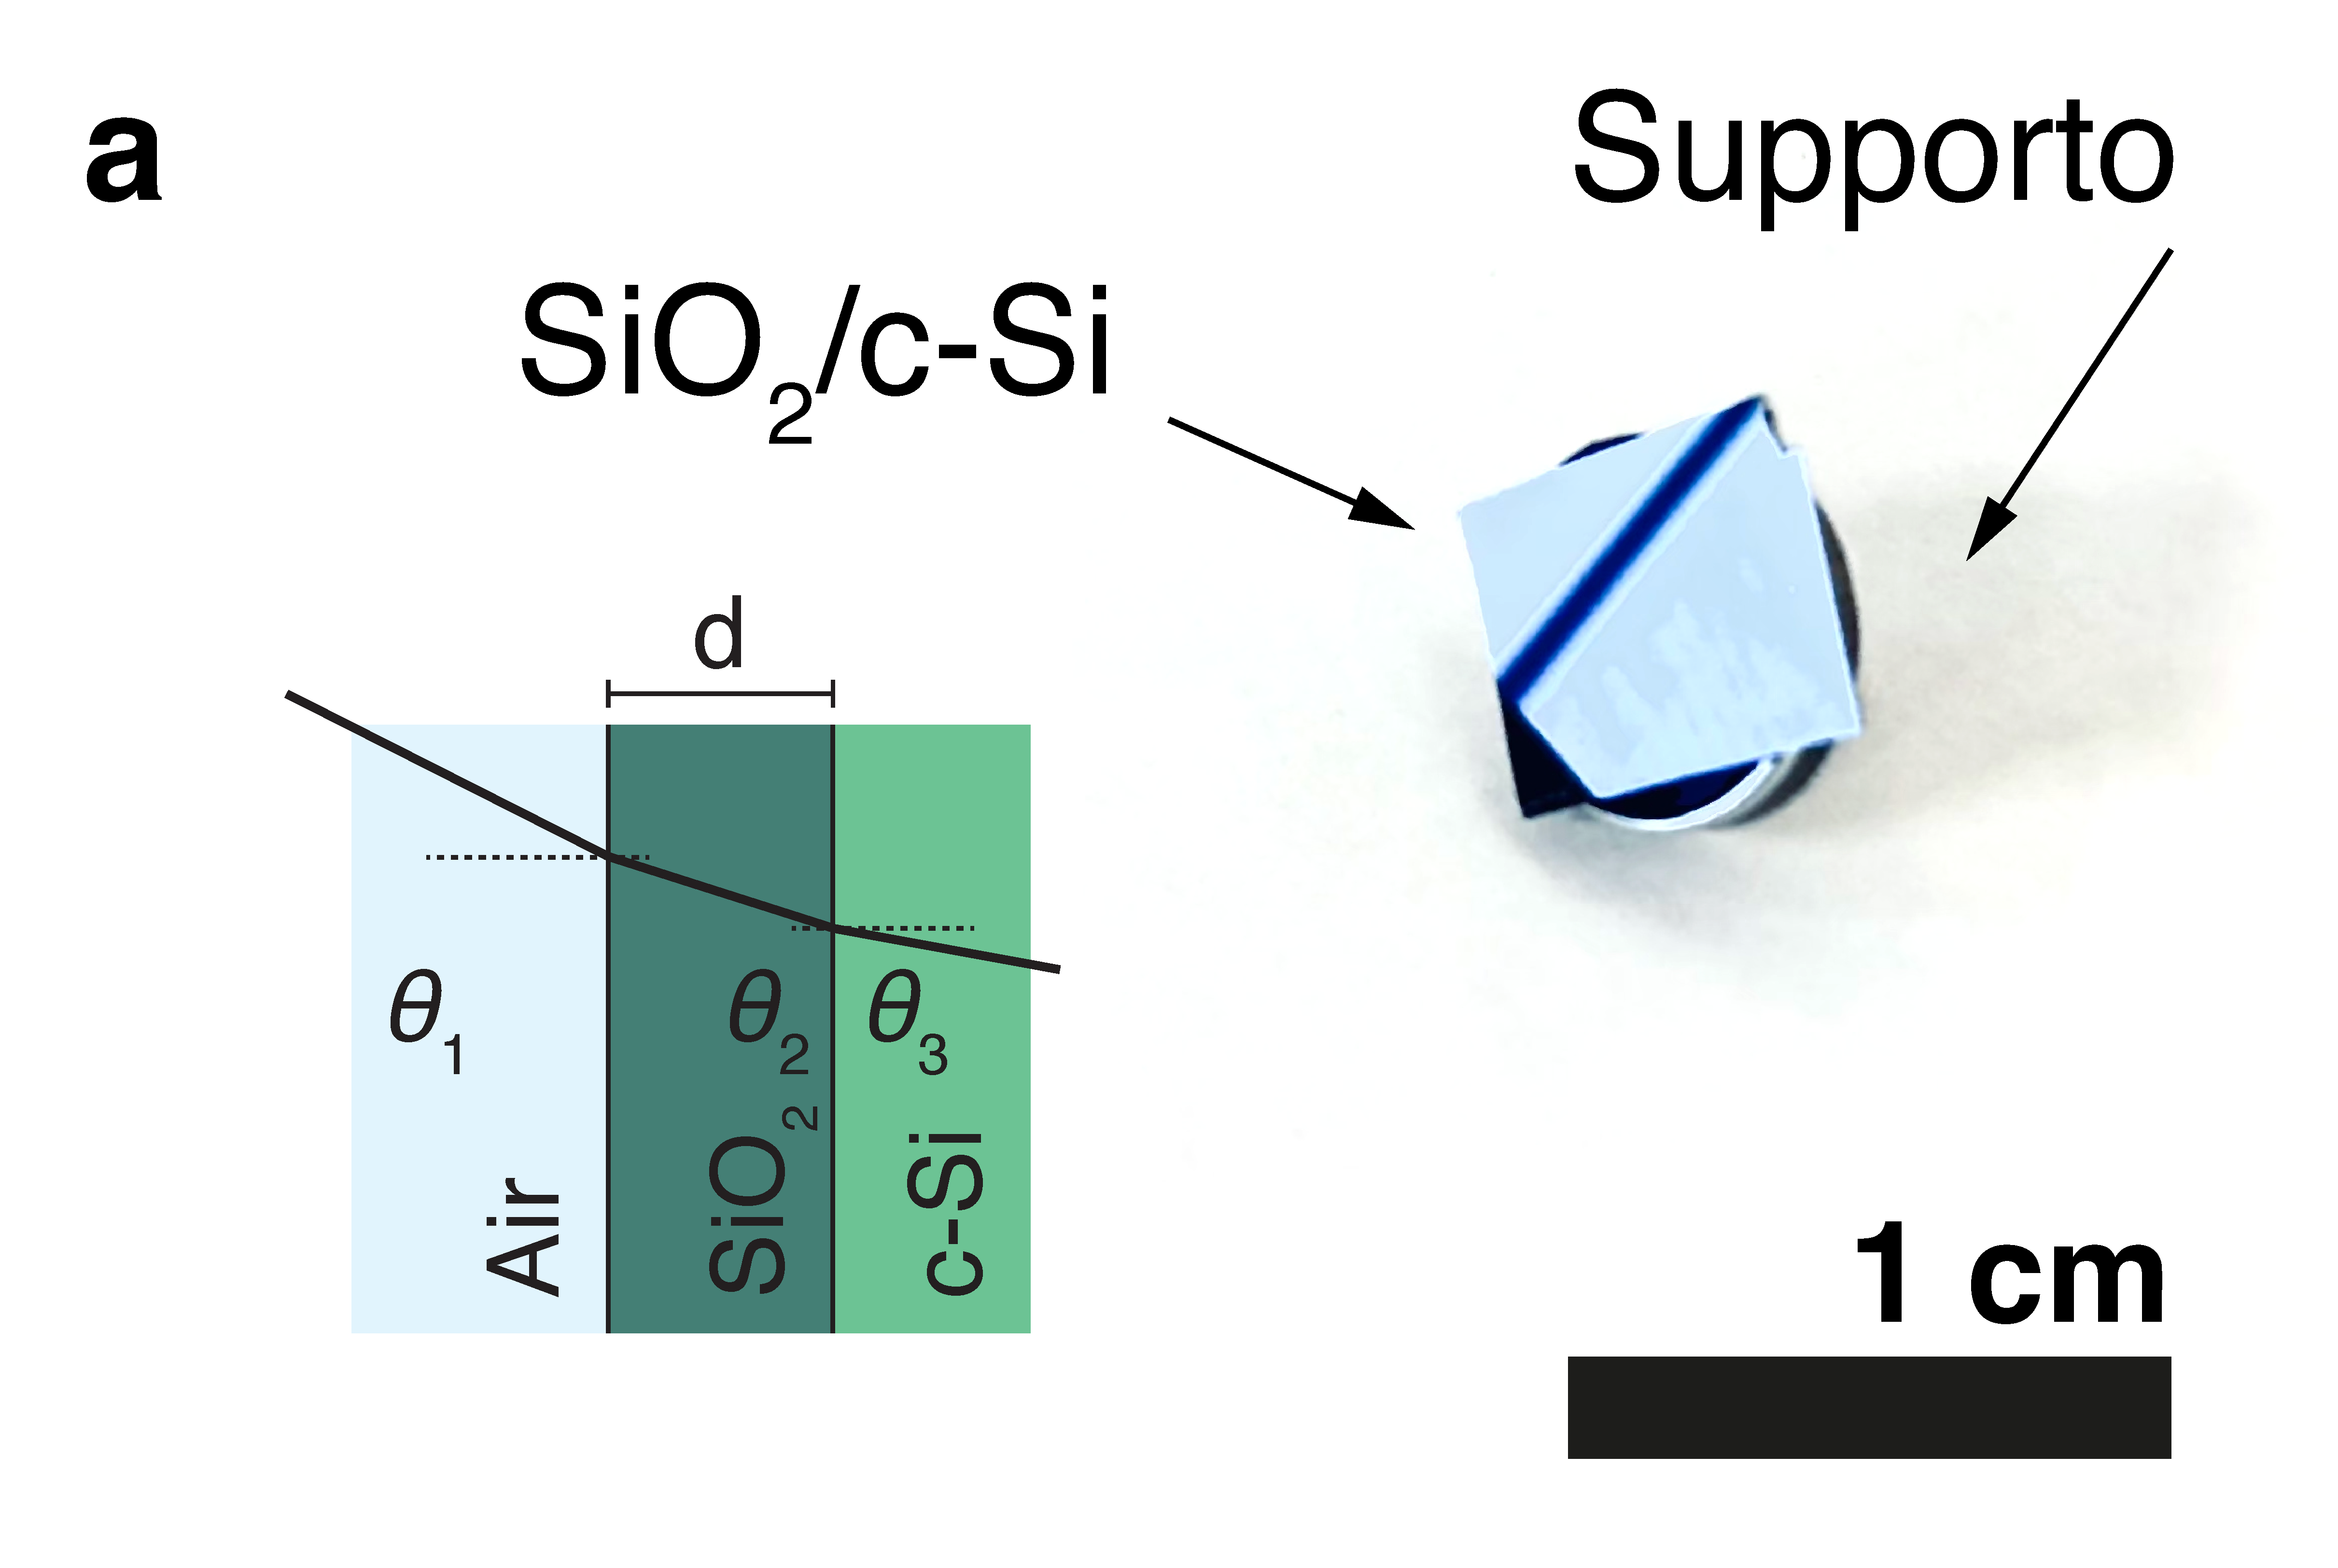
\includegraphics[width=0.4\linewidth,trim={0 4cm 0 0}]{figures/c-Si.pdf}\label{fig:c-Si}}
    \subfloat{\includegraphics[width=0.4\linewidth]{figures/Au_sample.pdf}\label{fig:Au}}
    \caption{\ref{sub@fig:c-Si} Campione di  cristallo di Silicio montato sul supporto necessario per poter effettuare le misure. A lato è anche schematizzata la struttura a layer dell'interfaccia del c-Si con l'aria, a cui è interposto un sottile strato di $\mathrm{SiO_2}$ che cambia quindi l'angolo con cui la luce incide sul silicio. \ref{sub@fig:Au} Campione di oro e schema della struttura dell'interfaccia aria/oro. Il campione è montato al centro del goniometro. Sullo stesso supporto è possibile anche fissare il campione di c-Si.}
    \label{fig:c-Si/Au_samples}
\end{figure*}

Ci possono essere però alcune situazioni in cui il modello semplificato non è sufficiente, sopratutto quando il materiale in questione, per quanto preparato con estrema precisione, presenta sottili strati superficiali di materiale con indice di rifrazione differente. Questo è vero in particolar modo per il cristallo di silicio, c-Si, per il quale si ha un deposito di ossido di silicio $\mathrm{SiO_2}$ (vedi figura \ref{fig:c-Si}) con uno spessore $d>\SI{1}{\nano\metre}$ sufficiente per avere fenomeni di riflessione multipla nel sottile film interposto ad ambiente (aria, con indice di rifrazione noto, $n_\mathrm{Air}$) e il substrato di c-Si, con indice $\underline n_\text{c-Si}$. La teoria che ne segue si complica. Dobbiamo allora introdurre il modello a tre fasi (\emph{three-phases model}\cite{cobetEllipsometrySurveyConcept2018, hinrichsEllipsometryFunctionalOrganic2018, yehOpticalWavesLayered1988})\footnote{Nel caso della ref. {\onlinecite{yehOpticalWavesLayered1988}} la convensione sul segno dell'esponenziale è differente da quella utilizzata invece dalla ref. {\onlinecite{hinrichsEllipsometryFunctionalOrganic2018}}, ma questo è indifferente considerato che l'esponenziale complesso è periodico $2\pi$. Nella \eqref{eq:three_phase_model} utilizziamo la convenzione presentata nella seconda} per cui i coefficienti introdotti in (\ref{eq:fresnel_rs}-\ref{eq:fresnel_rp}) non sono più sufficienti, ma dobbiamo introdurre i coefficienti \begin{equation}
    r = \frac{r_{al} + r_{ls}e^{2i\beta}}{1 + r_{al}r_{ls}e^{2i\beta}},\label{eq:three_phase_model}
\end{equation} valida sia per i modi TE che per i modi TM di oscillazione. I coefficienti $r_{al}$ e $r_{ls}$ hanno la stessa forma di (\ref{eq:fresnel_rs}-\ref{eq:fresnel_rp}), considerando questa volta che però gli angoli di incidenza sono relativi all'interfaccia che si sta considerando: aria/$\mathrm{SiO_2}$ nel caso di $r_{al}$, e $\mathrm{SiO_2}$/c-Si nel caso di $r_{ls}$. Il coefficiente $\beta$ è invece indicativo della differenza di fase legata al cammino ottico allinterno del layer sottile depositato sulla superficie del cristallo (si veda l'eq. (1.16) di ref. \onlinecite{hinrichsEllipsometryFunctionalOrganic2018}), ed è espresso come \begin{equation}
    \beta = \frac{2\pi}{\lambda} d \sqrt{\underline n_l^2 - \underline n_a^2 \sin^2\phi_a}.
\end{equation} Osserviamo subito che il modello è sicuramente più complesso del precedente, il che comporterà la necessità di fare assunzioni in fase di analisi dati per poter ottenere dei risultati corretti. 

\section{L'esperimento}

Descriviamo nel suo funzionamento e nelle scelte di progettazione l'esperimento, concentrandoci prima brevemente sul sistema ottico utilizzato, e quindi sulle scelte riguardanti il funzionamento e le caratteristiche dell'amplificazione e acquisizione del segnale, che consideriamo una prima analisi \emph{online} del dato ricevuto. Infatti dai differenti input che riceviamo passiamo quindi ad un dato \emph{pulito} che è più facile maneggiare. 

Del sistema ottico andiamo a definire le tre componenti principali, quali la sorgente utilizzata, il campione con il relativo supporto e il ricevitore/trasduttore, che permette di acquisire segnali in tensione dal segnale fisico. 

Dell'analisi online invece definiamo gli stadi principali come sono riportati in figura \ref{fig:lock-in/block_diagram}, e analizziamo le scelte di progettazione per assicurare il miglior funzionamento dell'esperimento. 

\subsection{Il sistema ottico}

L'esperimento è costituito da un goniometro da banco ottico con precisione di \ang{0;20} su entrambi gli angoli (incidenza e riflessione) rispetto al campione posizionato al centro. Il goniometro è assicurato ad un banco ottico sfruttato come supporto per l'intero setup, controllato localmente da un computer con LabView, che permette anche l'acquisizione dei dati. Uno dei due bracci del goniometro ospita il supporto per la sorgente laser, mentre l'altro ospita il fotodiodo rivelatore. Sul cammino ottico del fascio di luce è inoltre inserito un modulatore in frequenza, immediatamente vicino alla sorgente, e due filtri polarizzatori, posizionati dopo il \emph{chopper} ma prima del campione al centro del sistema. Quello più lontano dalla sorgente è l'ultima lente che il fascio attraversa prima di incidere sul campione, e definisce quindi il piano di polarizzazione dell'onda incidente. Quello immediatamente precedente è invece necessario per ridurre l'intensità della luce incidente sul campione e della frazione di luce che poi colpisce il fotodiodo per evitare una eccessiva usura del campione e dello strumento di misura, ed inoltre per non avere un segnale eccessivamente grande in ingresso sul sistema. La scheda di acquisizione è infatti limitata in ampiezza a circa \SI{10}{\volt}, per cui la scelta dell'angolo relativo tra le due lenti polarizzatrici è importante per poter controllare l'intensità secondo queste limitazioni sperimentali. Uno schema del setup utilizzato è in figura \ref{fig:setup}, mentre in figura \ref{fig:setup_on} troviamo una sua fotografia. 

\begin{figure*}
    \centering
    \subfloat{\includegraphics[height=5cm,page=1]{figures/setup.pdf}\label{fig:setup}}
    \subfloat{\includegraphics[height=5cm,page=2]{figures/setup.pdf}\label{fig:setup_on}}
    \caption{\ref{sub@fig:setup} Schema del setup utilizzato. $P_1$ è il primo polarizzatore, che controlla l'intensità del fascio, insiema a $P_2$, che inoltre permette di definire la polarizzazione della luce, ricordando che l'intensità dopo due filtri è proporzionale al $\cos\theta_{1,2}$ dell'angolo compreso tra i due filtri. \ref{sub@fig:setup_on} Fotografia dell'esperimento completo durante una misura. Si può facilmente vedere il sottile fascio laser in uscita dalla sorgente, che attraversa il disco del chopper e poi due lenti polarizzatrici. Il fotodiodo è pure visibile. Il campione è nascosto invece dal supporto posto al centro del goniometro. }
    \label{fig:setup_and_photo}
\end{figure*}

\paragraph*{Sorgente} La sorgente è costituita da un laser verde estremamente collimato, alimentato in corrente continua. La luce emessa ha una lunghezza d'onda precisa e sufficientemente stabile a \SI{532}{\nano\metre}. Non essendo possibile alternare l'emissione del laser elettronicamente, allora possiamo modularne il segnale meccanicamente. Introduciamo allora un chopper meccanico che lavorando su un motore elettrico in corrente continua può modulare il segnale con una frequenza che può andare da \SI{1}{\hertz} fino a \SI{4}{\kilo\hertz}. La scelta della frequenza con cui moduliamo il segnale è allora dettata dalle caratteristiche in spettro del rumore di fondo. 

\begin{figure}
    \centering
    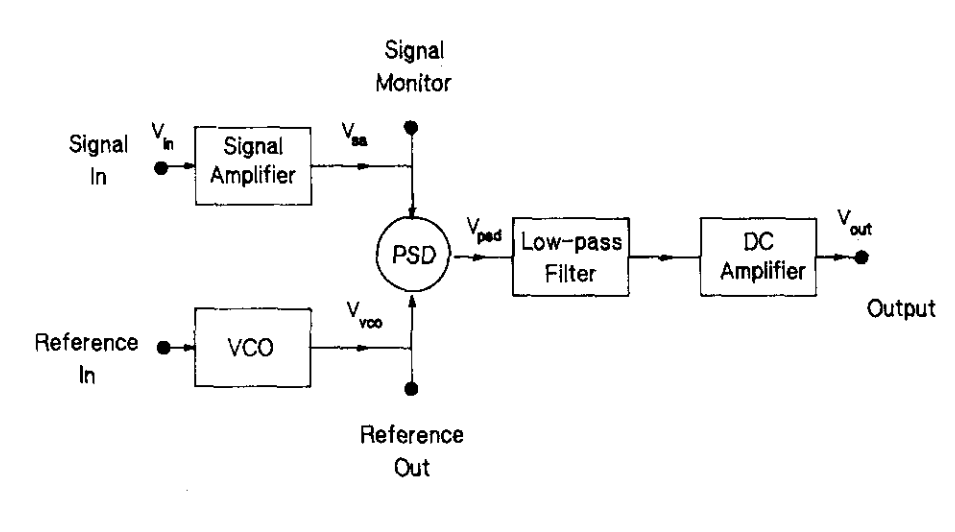
\includegraphics[width=\linewidth]{figures/block_diagram.png}
    \caption{Diagramma a blocchi del lock-in. Dall'alto abbiamo un primo stadio di amplificazione; sotto l'ingresso per il segnale di riferimento; \textsc{psd}: allineamento in fase e raddrizzamento del segnale amplificato sul riferimento. \textsc{adc}: convertitore analogico-digitale, scheda di acquisizione National Intruments BNC-2120. Il segnale è così fatto passare su un filtro passa basso implementato digitalmente. }
    \label{fig:lock-in/block_diagram}
\end{figure}

Il chopper permette di misurare la frequenza del segnale prodotto e la fornisce su una linea di uscita TTL. Questa quindi può essere utilizzata come referenza in ingresso allo stadio centrale del lock-in (figura \ref{fig:lock-in/block_diagram}) ed è inoltre letta in ingresso alla scheda di acquisizione per verificare che la frequenza sia costante nel tempo. L'errore che viene rilevato è inferiore a $0.5\%$, osservando solo variazioni sui decimi di \si\hertz, su un segnale a $\SI{2745}\hertz$ su tutte le acquisizioni. Queste fluttuazioni sono sufficientemente piccole per poter considerare eventuali effetti sul segnale in uscita dal lock-in trascurabili. 

Il fascio luminoso in uscita dalla sorgente è allineate per incidere ortogonalmente sulle lenti polarizzatrici, e inoltre per incidervi centralmente, così da poter trascurare possibili effetti di bordo. 

\paragraph*{Il campione} Si utilizzano per realizzare la misura due campioni differenti, un primo costituito da un cristallo di silicio, che indichiamo con c-Si, e un secondo dato da una sottile lamina di oro, che indichiamo con il simbolo Au. Si tratta di campioni sufficientemente lisci, in particolare il campione di c-Si, che non presenta deformazioni notevoli sulla superficie, e sopratutto di materiali conduttori, come nel caso dell'Au, o semiconduttori, come nel caso del c-Si. Questo come detto prima implica la presenza di un coefficiente di assorbimento indicato con $\kappa_\text{Au/c-Si}$. 

Il campione è montato su un sostegno centrato rispetto al goniometro, con la possibilità di muoversi lungo gli assi $x$, $y$ e $z$ locali, dove indichiamo l'asse $z$ come l'asso normale alla superficie del campione, e $x, y$ gli assi della terna destrorsa che indicano spostamento nella direzione verticale al piano del banco ottico e di spostamento laterale. In questo modo è infatti possibile spostare in tre dimensioni il campione, per fare in modo che il punto in cui è colpito dal fascio luminoso sia sempre invariato. Possiamo compiere questa verifica fissando le direzioni $x$ e $y$, e andando a variare la posizione lungo $z$, facendo in modo che piccole rotazioni del supporto sull'asse verticale non facessero variare la posizione dello spot di incisione del fascio luminoso. Questo controllo viene eseguito ogni giorno e ogni volta che il campione è cambiato. Il supporto può accogliere il campione tramite un incastro standard, che permette di poter intercambiare facilmente il materiale presente. 

Consideriamo inoltre che i materiali utilizzati non siano estremamente esotici nella loro costituzione, per cui possiamo inoltre supporre che nella riflessione la frequenza della luce incidente non sia cambiata, per fenomeni di riflessioni multiple o per splitting di un'onda multicomponente. Possiamo fare queste assunzioni fondandoci su alcune considerazioni importanti
\begin{enumerate}
    \item Il campione, anche nel caso del c-Si, dove è presente un sottile film di $\mathrm{SiO_2}$, è comunque sufficientemente liscio, e sufficientemente sottile per poter trascurare eventuali riflessioni multiple. 
    \item Il passo del cristallo, sia del c-Si che per l'Au, è non comparabile in termini di ordini di grandezza con la costante reticolare, che sono\cite{BasicParametersSilicon2023, CODATAValueLattice, daveyPrecisionMeasurementsLattice1925, MaterialsDataAu2020, MaterialsDataSi2020, NSMArchivePhysical} \begin{align*}
        &\SI{5.431 020 511(89)e-10}{\metre}\quad\text{per c-Si}\\
        &\SI{4.065+-0.004e-10}{\metre}\quad\text{per Au},
    \end{align*} praticamente trascurabili rispetto alla lunghezza d'onda del laser utilizzato, \SI{532e-9}{\metre}.
    \item Infine possiamo considerare che il laser sia estremamente monocromatico, producendo un fascio solo ad una lunghezza d'onda definita. 
\end{enumerate} Queste considerazioni possono tranquillamente farci assumere che anche se ci sono delle variazioni in frequenza, queste sono trascurabili percentualmente. 

\paragraph*{Il ricevitore} L'ultima componente del setup è dato da un fotodiodo, utilizzato come ricevitore (\textsc{Laser-Optronic}/detector mod. 260). È anche questo assicurato al goniometro, con un supporto ad anello, come si può vedere in figura \ref{fig:photo-diode}, e può muoversi quindi lungo la circonferenza con centro sul punto in cui è fissato il campione. Ha una precisione su supporto che va come per tutto il goniometro a \ang{0;20}. In realtà la superficie sensibile del fotodiodo, il singolo pixel semiconduttore, ha una larghezza che copre più di un terzo di grado, come sempre possiamo vedere nella figura \ref{fig:photo-diode}, dove oltre ad osservare che l'apertura effettiva angolare del fotodiodo è maggiore della sensibilità angolare del goniometro, la risposta in termini di tensione è costante su tutta la larghezza, fatta eccezione per i fenomeni di bordo, dove però possiamo osservare una riduzione del segnale legato alla forma del laser che non è uniforme in potenza su tutta la superficie incidente ma diffusa sui bordi, come si può vedere nelle regioni evidenziate in verde. 

Otteniamo allora che la precisione angolare complessivamente può essere considerata di circa \ang{2}, circa sei volte la precisione sul goniometro. Questo rende comunque l'incertezza sugli angoli inferiore all'incertezza che invece abbiamo sui valori di tensione e quindi sui coefficienti di riflessione. Questo può quindi permetterci di semplificare il modello andando poi a costruire una unica funzione da minimizzare che risulta essere più semplice rispetto a dover considerare anche incertezze sugli angoli. Discuteremo più avanti queste considerazioni, andando a vedere se possono avere inficiato in qualche modo i risultati ottenuti. 

\begin{figure}
    \centering
    \includegraphics[width=\linewidth,trim={0 8cm 0 0}]{figures/photoDiode.pdf}
    \caption{Immagine del fotodiodo utilizzato per la acquisizione dei dati. Il laser colpisce ortogonalmente il cristallo semiconduttore , che ha una apertura angolare di circa \SI{2}{\degree}, sulla quale la risposta è pressoché uniforme, come possiamo dedurre anche dal grafico, ad eccezione fatta per le regioni ai bordi, evidenziate in verde, per le quali interviene il fattore di forma del fascio di luce laser, che per quanto estremamente collimato presenta una distribuzione approssimativamente gaussiana, della quale stiamo osservando le code.}
    \label{fig:photo-diode}
\end{figure}

\begin{figure}
    \centering
    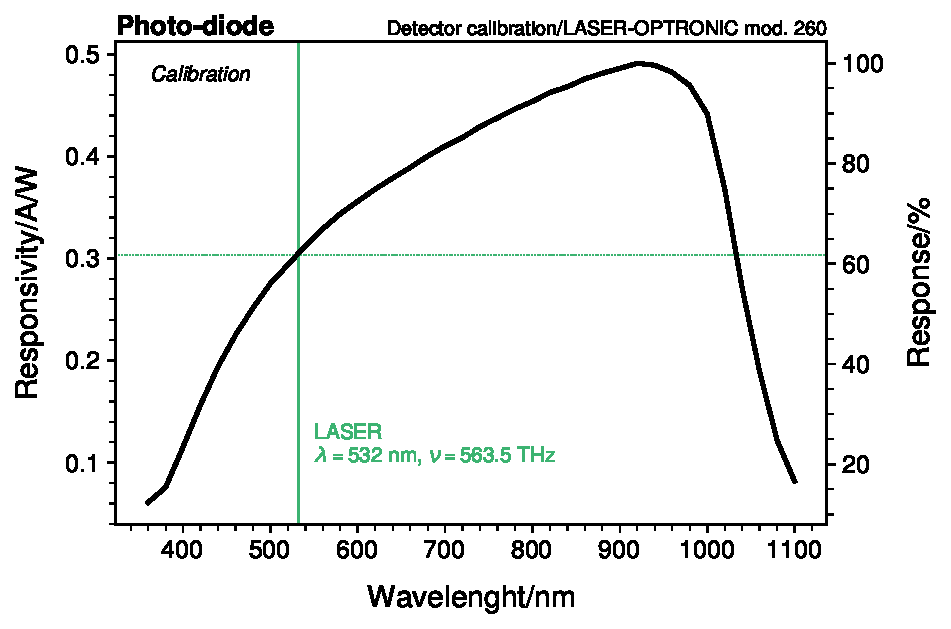
\includegraphics[width=\linewidth]{figures/detector_calib.pdf}
    \caption{Calibrazione del fotodiodo, nel range \SI{360}{\nano\metre}-\SI{1100}{\nano\metre}. Il laser utilizzato è corrispondente a \SI{532}{\nano\metre}, a cui corrisponde una risposta di $\SI{0.303}{\ampere\per\watt}\simeq\SI{61.7}{\%}$. Considerando sempre la stessa frequenza del laser possiamo in generale non preoccuparci dell'efficienza ridotta dell'accoppiamento di fotodiodo con il laser considerato.}
    \label{fig:detector_calib}
\end{figure}

Il sensore è anche caratterizzato in efficienza rispetto alla lunghezza d'onda della luce incidente, con la curva riportata in fig. \ref{fig:detector_calib}. La regione in cui il laser produce è centrata a \SI{532}{\nano\metre}, con una incertezza trascurabile. Per questa lunghezza d'onda la risposta del pixel corrisponde a circa \SI{0.303}{\ampere\per\watt}, che in termini di efficienza di risposta corrisponde ad una efficienza del \SI{61.7}{\%} circa. Questo però è un problema per quanto già detto in precedenza commentando i campioni utilizzati, in quanto la lunghezza d'onda della luce incidente sul sensore è sempre uguale, a meno di variazioni trascurabili, anche rispetto alla curva di risposta al sensore riportata in figura. Infatti per una variazione della lunghezza d'onda di circa \SI{20}{\nano\metre}, corrispondente a circa una variazione del \SI{3.75}{\%} della lunghezza d'onda del laser, abbiamo una variazione in intensità corrispondente a circa \SI{0.018}{\ampere\per\watt}, corrispondente ad una variazione massima del \SI{3.8}{\%}. Possiamo quindi trascurare anche questa possibile fonte di errore, ipotizzando, per le ragioni sopracitate, che la lunghezza d'onda abbia variazioni dell'ordine delle decine di nanometri, e che quindi l'incertezza del \SI5\% sia trascurabile. 

Vogliamo anche caratterizzare in frequenza elettronica il segnale che riceviamo dal fotodiodo, per cui acquisiamo tre sequenze da 1 secondo che componiamo in una sequenza da tre secondi di dati lasciando tutto il sistema acceso (e quindi anche la parte di amplificazione del segnale del fotodiodo, che descriviamo nel prossimo paragrafo) fatta eccezione per il laser, che non viene puntato sul campione. Possiamo quindi eseguire uno spettro di densità di potenza del segnale ottenuto utilizzando il metodo introdotto da Welch\cite{welchUseFastFourier1967a}, eseguendo \emph{fast Fourier transforms}, FFT,  del segnale, che dividiamo in sequenze da \SI{0.5}{\second} e sovrapponiamo per metà, compiendo delle medie. Lo spettro così ottenuto è riportato in fig. \ref{fig:NDS}. Sono anche riportati gli spettri di densità delle singole sequenze di un secondo, che presentano le stesse caratteristiche dello spettro combinato. In scala logaritmica possiamo osservare un primo picco alla frequenza di \SI{100}{\hertz}, e le successive armoniche di ordine dal 2 al 6, ben visibili, corrispondenti al segnale elettrico di rete. 

Per questo decidiamo allora di operare la modulazione del segnale luminoso ad una frequenza di circa \SI{2.7}{\kilo\hertz}, che sia distante dalle prime armoniche del segnale di rete e facciamo in modo che sia non multiplo interno della frequnza di rete per spostarci da eventuali effetti di rumore. In questo modo potremo poi anche pensare di valutare il rapporto tra rumore e segnale (SNR). 



\begin{figure}
    \centering
    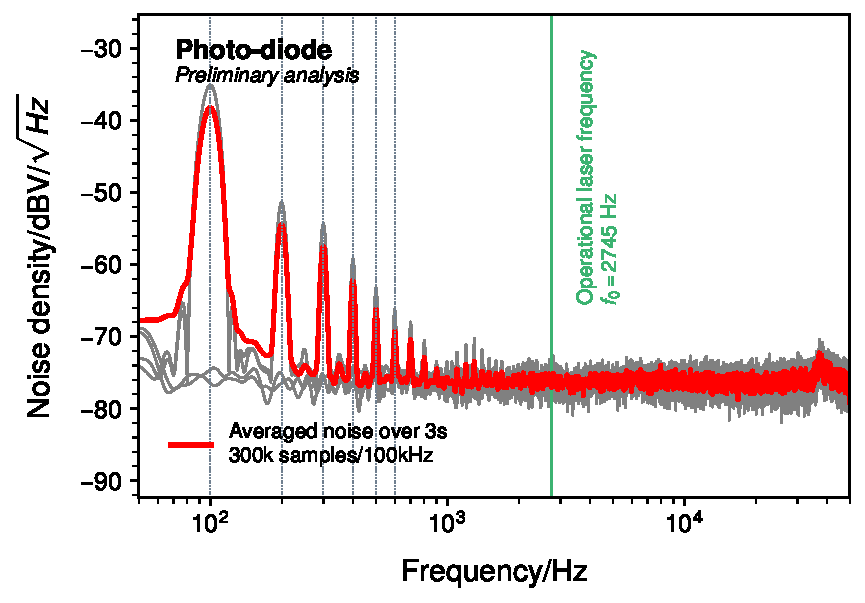
\includegraphics[width=\linewidth]{figures/noise_nds.pdf}
    \caption{Spettro di densità\cite{welchUseFastFourier1967a} del rumore elettronico ottenuto da \SI{3}{\second} di dati, con \emph{Fast Fourier Transform, FFT,} di \SI{0.5}{\second}. Osserviamo la presenza dell'armonica principale a \SI{100}{\hertz}, e le armoniche di ordine da 2 a 9 sufficientemente distinte. La frequenza di operazione dell'esperimento è invece spostata de tale regione, ed è evidenziata dalla linea verde, a \SI{2745}{\hertz}.}
    \label{fig:NDS}
\end{figure}

\subsection{Lock-in, analisi online preliminare}

La rappresentazione a blocchi del lock-in\cite{scofieldFrequencydomainDescriptionLockin1994} riportata in figura \ref{fig:lock-in/block_diagram} è schematica ma indicativa del flusso che il segnale compie dal momento in cui è convertito dal fotodiodo a quando poi viene infine salvato. 

Dal trasduttore il segnale elettrico viene amplificato su un amplificatore per strumentazione con guadagno combinato sui due stadi separati di circa $G_\mathrm{amp}=\SI{0.1}{K}/\SI{1}{K}$. La scelta del guadagno viene fatta assieme alla scelta dell'angolo compreso tra i piani di polarizzazione di $P_1$ e $P_2$ (figura \ref{fig:setup}) per fare in modo che ci sia un ottima efficienza di amplificazione rispetto al rumore, ma anche considerando che il segnale così posto in ingresso alla scheda di acquisizione non vada oltre il limite consentito di $\pm\SI{10}{\volt}$. 

In parallelo dal chopper abbiamo in uscita un segnale TTL standardizzato che possiamo dare in input allo sfasatore (\textsc{vco} in figura \ref{fig:lock-in/block_diagram}). 

Questi due segnali si accoppiano al centro del lock-in dove il primo è rettificato sul secondo, utilizzato come referenza, e quindi risulta essere un segnale praticamente in continua. Questo purtroppo non avviene perché come accennato all'inizio il segnale che si utilizza come referenza non è un segnale sinusoidale, che quindi presenta solo una frequenza corrispondente all'armonica principale, ma invece è un segnale dato da un'onda quadra, che quindi presenta anche armoniche successive, che portano quindi ad avere effetti a frequenze maggiori. Per ovviare a questo problema introduciamo allora un filtro passa basso, che però implementiamo digitalmente con LabView dopo aver convertito il segnale. 

La conversione del segnale avviene attraverso la scheda di acquisizione National Instrument BNC-2120, che presenta alcune caratteristiche limitanti già citate. Innanzitutto su ogni ingresso abbiamo un limite all'ampiezza di \SI{10}{\volt}, che possono essere riferiti a terra o riferiti ad un altro ingresso. Avendo tutto il sistema posto a massa e la massa posta a terra possiamo fare misure riferite a terra. La frequenza di campionamento della scheda è limitata a \SI{250}{kilo~samples\per\second} distribuita su tutti i canali, che limita su due canali di acquisizione ogni canale ad una frequenza di \SI{100}{\kilo\hertz}. Questo implica anche una risoluzione di circa $1/(\num{100e3})=\SI{1e-5}{\hertz}$ sulla FFT, con una acquisizione di \SI{1}{\second}. 

Il segnale digitale è quindi filtrato su un filtro passa basso con frequenza di taglio corrispondente a $f_\mathrm{cut}=\SI{200}{\hertz}$, per fare in modo che solo il segnale in continua sia preservato, e invece tutte le successive armoniche (che corrispondono ai multipli interi di $f_0=\SI{2745}{\hertz}$) siano ridotte e rese trascurabili. 

Il dato così ottenuto è quello che alla fine può essere salvato, corrispondente, a meno di costanti, in prima approssimazione con una relazione lineare, al valore di intensità, espressa in Watt, della luce incidente. 




%%%%%% TODO
\iffalse
\begin{figure*}
    \centering
    \subfloat[]{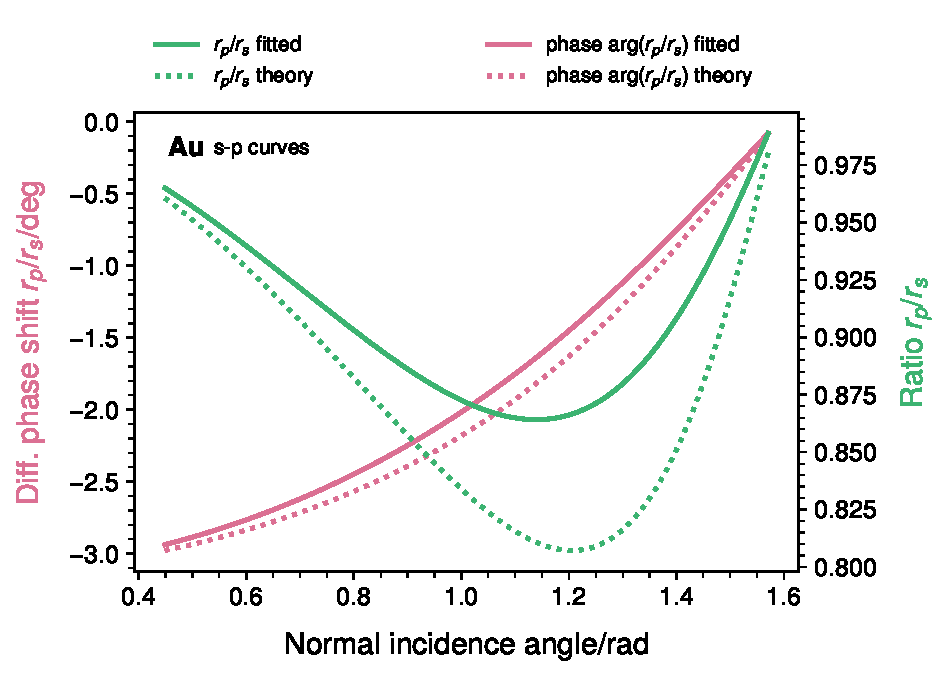
\includegraphics[width=0.45\linewidth]{figures/phase_ratio_Air.Au.pdf}\label{fig:Air.Au.rp/rs}}
    \subfloat[]{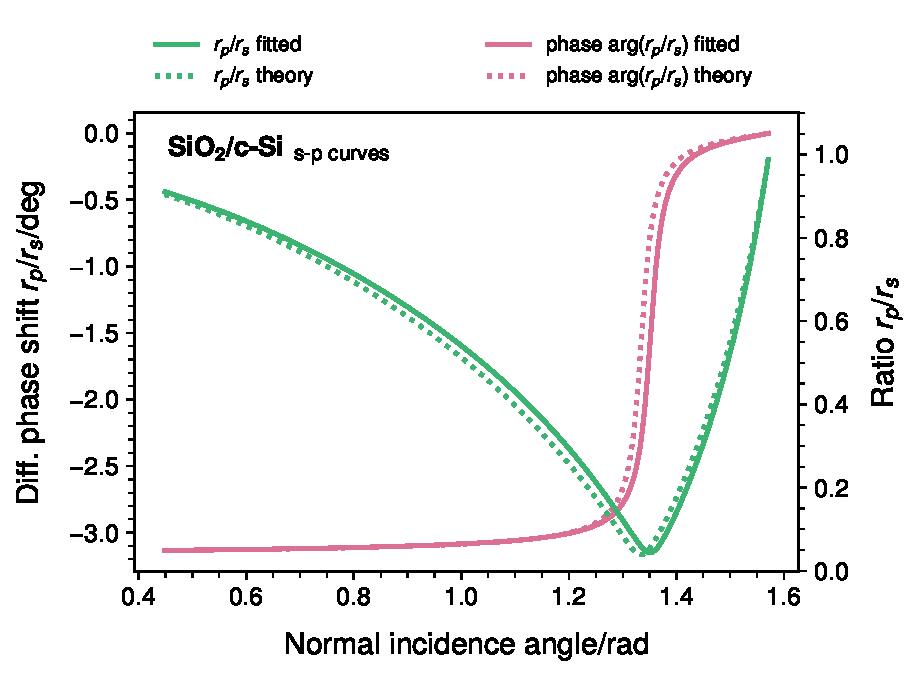
\includegraphics[width=0.45\linewidth]{figures/phase_ratio_Air.SiO2.Si.pdf}\label{fig:Air.SiO2.Si.rp/rs}}
    \caption{\ref{sub@fig:Air.Au.rp/rs}\ref{sub@fig:Air.SiO2.Si.rp/rs}}
    \label{fig:enter-label}
\end{figure*}
\fi

\appendix

\bibliography{references/brewster_research}

\end{document}
